% !TEX root = ../../../main.tex
% 来源：高中物理甲种本·第三册（电磁·光学·近代物理）
% 章节：交流电 / 三相交流电
% 原始文件：3.tex，行 1541-1577
% 类型：tikz
% ---
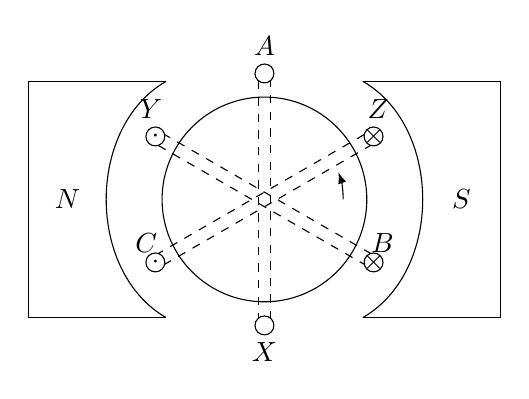
\begin{tikzpicture}[>=latex]
\draw (0,0) circle (1.3);

\foreach \x in {30,90,150}
{
    \draw [rotate=\x, dashed] (-1.6,-.08) rectangle (1.6,.08);
}
    \foreach \x in {30,90,150}
{        
    \draw (\x:1.6) [fill=white] circle (0.12);
    \draw (-\x:1.6) [fill=white] circle (0.12);
}

\node at (30:1.6){$\times$};
\node at (-30:1.6){$\times$};
\node at (150:1.6){$\cdot$};
\node at (-150:1.6){$\cdot$};

\draw [->] (1,0) arc (0:20:1);
\node at (32:1.7)[above]{$Z$};
\node at (-28:1.7)[above]{$B$};
\node at (150-2:1.7)[above]{$Y$};
\node at (-150-2:1.7)[above]{$C$};
\node at (90:1.7)[above]{$A$};
\node at (-90:1.7)[below]{$X$};

\draw (3,1.5)--(1.25,1.5);
\draw (3,-1.5)--(1.25,-1.5);
\draw (1.25,1.5) to [bend left=60](1.25,-1.5);
\draw (3,1.5)--(3,-1.5);
\draw (-3,1.5)--(-3,-1.5);
\draw (-3,1.5)--(-1.25,1.5);
\draw (-3,-1.5)--(-1.25,-1.5);
\draw (-1.25,1.5) to [bend left=-60](-1.25,-1.5);
\node at (-2.5,0){$N$};\node at (2.5,0){$S$};

\end{tikzpicture}
